\documentclass{beamer}

\usetheme{Berlin}
\usecolortheme{beaver}
\usepackage{amssymb}
\usepackage{graphicx}

\title{Napredna računalniška orodja\\ (Prva domača naloga)}
\author{Alen Planinšec\\ 23211290}
\date{\today}

\titlegraphic{
    
\includegraphics[width=2cm]{slike/fs_logo.png}}

\begin{document}

\titlepage

\begin{frame}
\frametitle{Kazalo}
\tableofcontents
\end{frame}

\section{Približek števila $\pi$ z metodo Monte Carlo}
\begin{frame}
  \frametitle{Definicija naloge}
  Z metodo Monte Carlo smo v programu Matlab izračunali približno vrednost števila $\pi$.\\ Postopek domače naloge:
     \begin{itemize}
        \item definicija funkcijske datoteke s funkcijo \texttt{mcc\_pi.m} z enim vhodnim parametrom (število naključnih točk n),
        \pause
        \item programska datoteka \texttt{calc\_pi.m}, ki vključuje prejšnjo funkcijsko datoteko in novo funkcijo, ki primerja število točk znotraj in zunaj kroga in tako oceni vrednosti $\pi$ in odstopanje od prave vrednosti,
        \pause
        \item vključitev anonimne funkcije za izris loka krožnice,
        \pause
        \item vizualizacija točk znotraj in zunaj krožnice
  \end{itemize}
\end{frame}

\section{Funkcijska in programska datoteka}
\begin{frame}
    \frametitle{Funkcijska datoteka}
            \item Funkcijska datoteka ima enako ime kot prva funkcija v datoteki.
            \pause
            \item Spremenljivke v tovrstni datoteki so lokalne in niso dostopne iz drugih funkcij. 
            \pause
            \item Ta del programa za izračun razvijemo v obliki funkcijske datoteke z imenom \texttt{mcc\_pi.m}, ki ima en vhodni parameter (število točk n). 
            \pause
            \item Funkcija ob klicu vrne posebej koordinate točk znotraj in zunaj kroga.
 \begin{figure}
    \centering
    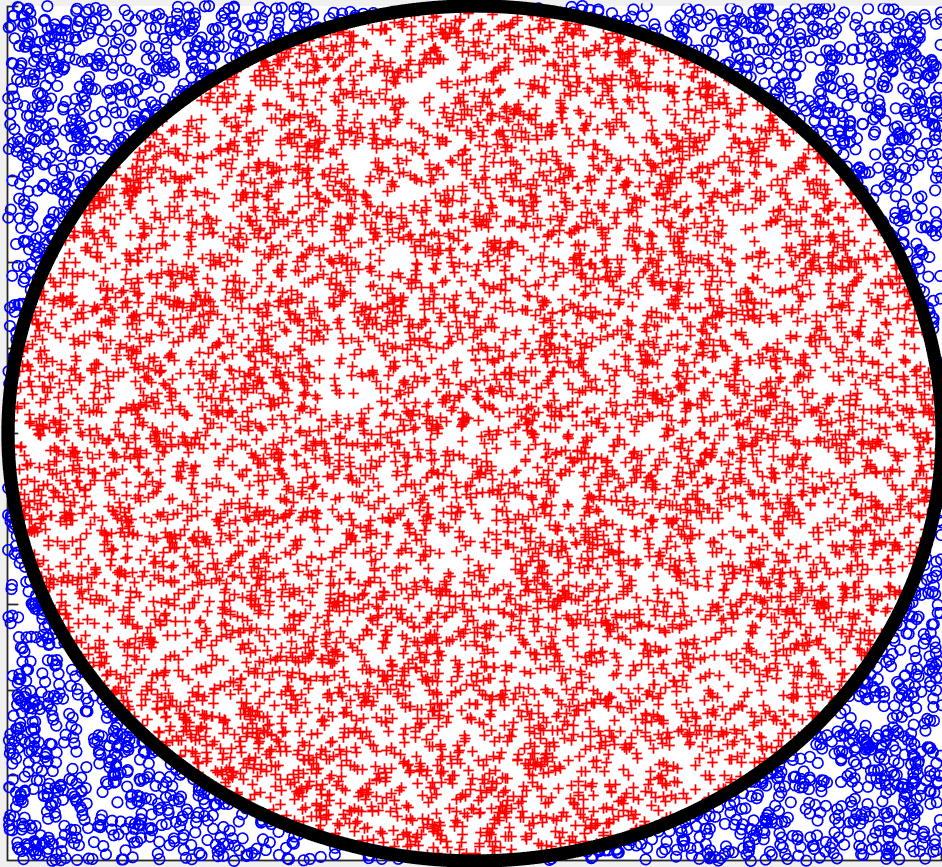
\includegraphics[width=0.3\textwidth]{slike/10 000 točk.png}
  \end{figure}
\end{frame}

\begin{frame}{Programska datoteka}
    \item Programska datoteka je običajno krovna datoteka, ki definira začetne vrednosti
    in kliče funkcije potrebne za rešitev problema.
    \pause
    \item V našem primeru je to \texttt{calc\_pi.m}.
\end{frame}

\begin{frame}{Koordinate naključnih točk}
Točke znotraj kroga in kvadrata lahko izrišemo.
Na zadnji strani so prikazi izrisa za različne vhodne parametre števila točk.
\begin{figure}
\end{figure}
\end{frame}

\section{Vizualizacija}
\begin{frame}{Vizualizacija rezultatov}
    Kot rezultat dobimo ocenjeno vrednost števila $\pi$ in napako pri računanju.  S spreminjanjem števila naključnih točk $n$ ugotovimo, da je z večjim številom točk napaka vedno manjša. \\
    \pause
    Prikaz za n=10 000 in n=100 000
\begin{figure}
  \begin{minipage}{0.5\textwidth}
    \centering
    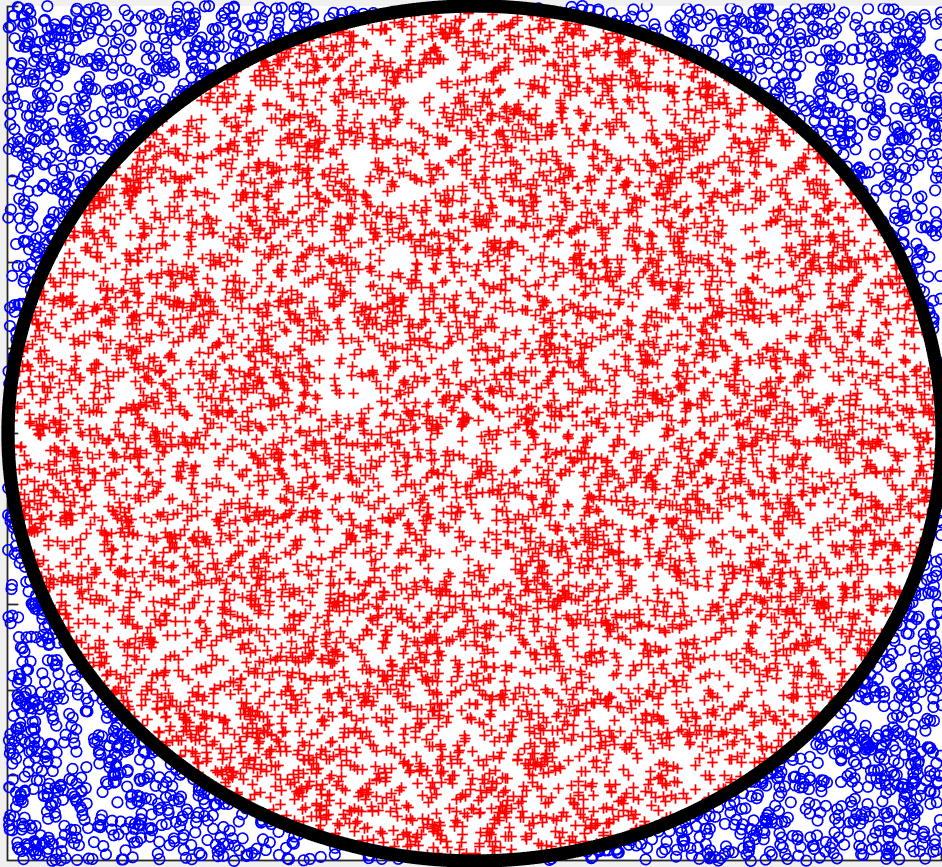
\includegraphics[width=1\textwidth]{slike/10 000 točk.png}
  \end{minipage}\hfill
  \pause
  \begin{minipage}{0.45\textwidth}
    \centering
    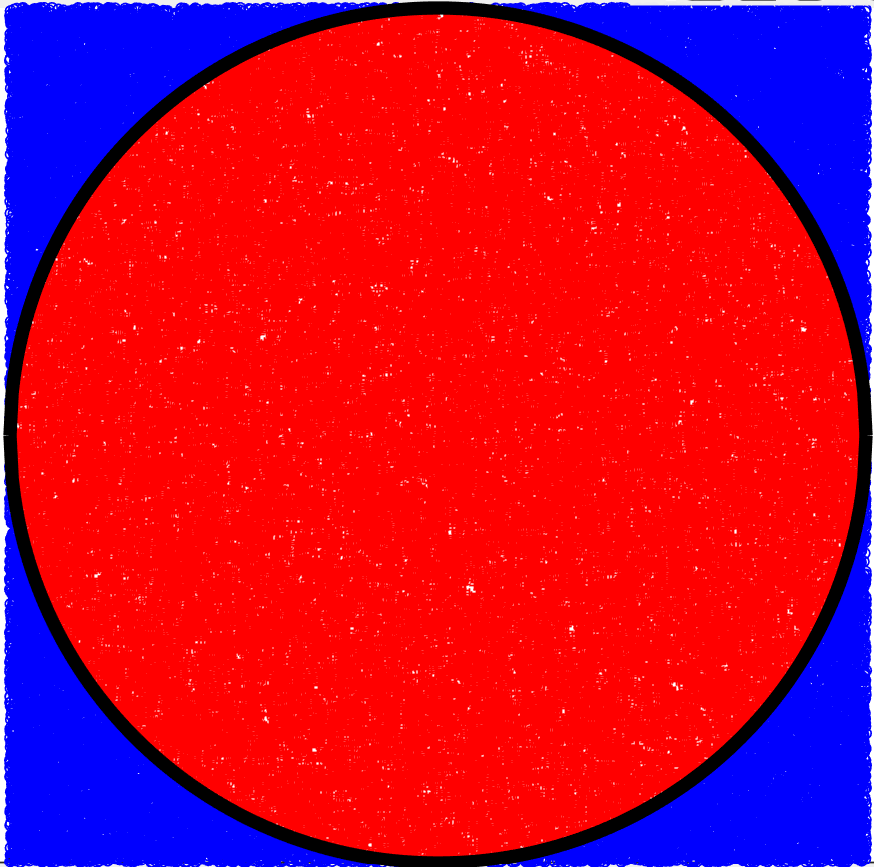
\includegraphics[width=1\textwidth]{slike/100 000 točk.png}
  \end{minipage}
\end{figure}

\end{frame}

\end{document}